\documentclass{article}
\usepackage[utf8]{inputenc}
\usepackage{titling}
\usepackage{graphicx}
\usepackage{xcolor}
\usepackage[colorlinks=true,linkcolor=darkgray, urlcolor =gray]{hyperref}
\usepackage[spanish]{babel}
\DeclareUnicodeCharacter{301}{~}
\usepackage{url}
\DeclareUnicodeCharacter{202F}{\,}


\title{Práctica WLAN: Parte 1}
\author{Cristina Díaz García}
\date{Noviembre 2018}

\renewcommand\maketitlehooka{\null\mbox{}\vfill}
\renewcommand\maketitlehookd{\vfill\null}


\begin{document}

\addcontentsline{toc}{section}{Índice general}

\begin{titlingpage}
\maketitle

\begin{center}

\includegraphics[scale=0.4]{WLAN/wireshark.jpg} 
\end{center}

\end{titlingpage}

\newpage

\tableofcontents

\newpage

\section{Quiz 1}

Se está accediendo a la página \textit{en.wikipedia.org}, pasando por \textit{wikimedia} y \textit{pagead2.googlesyndication.com}.

\begin{center}
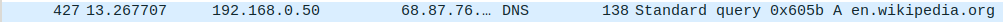
\includegraphics[scale=0.4]{WLAN/wikipedia.png} %427
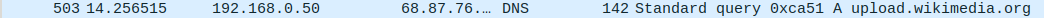
\includegraphics[scale=0.4]{WLAN/wikipedia3.png} %503
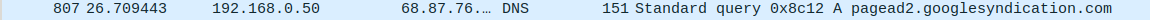
\includegraphics[scale=0.4]{WLAN/pagead2.png} %807
\end{center}

\begin{center}
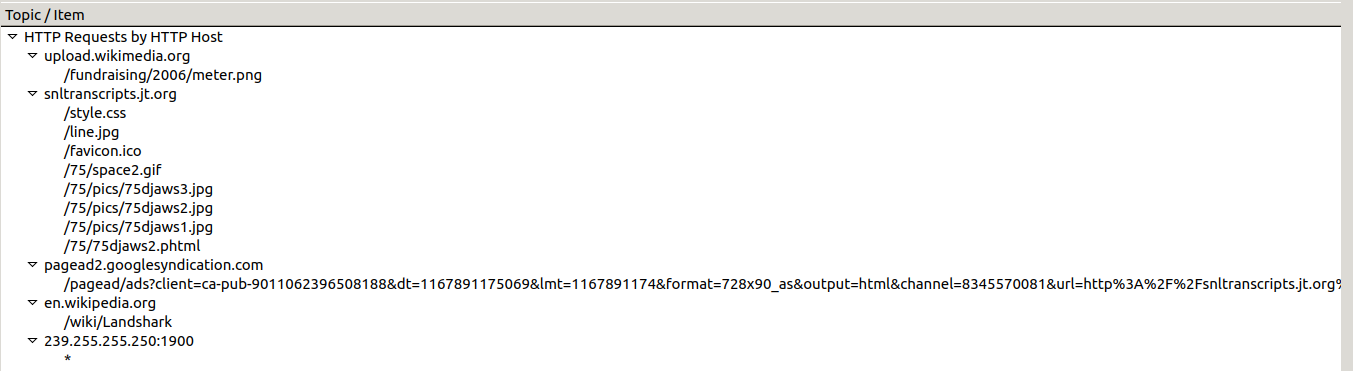
\includegraphics[scale=0.3]{WLAN/trafico.png}
\end{center}

\section{Quiz 2}

La señal más baja es aquella de la que más se pierde la señal, y mientras más mayor el valor absoluto del RSSI negativo, mayor es la pérdida de señal.

\begin{center}
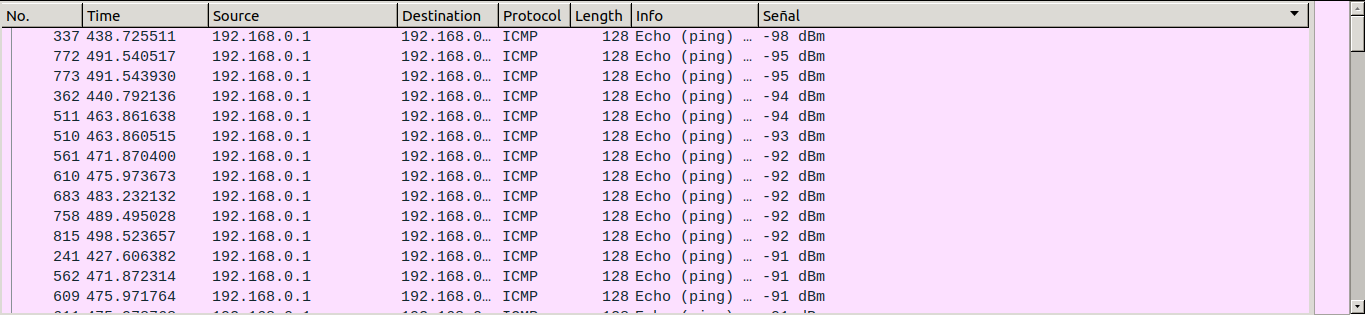
\includegraphics[scale=0.3]{WLAN/signal.png} 
\end{center}

La gráfica de la evolución temporal es la siguiente:

\begin{center}
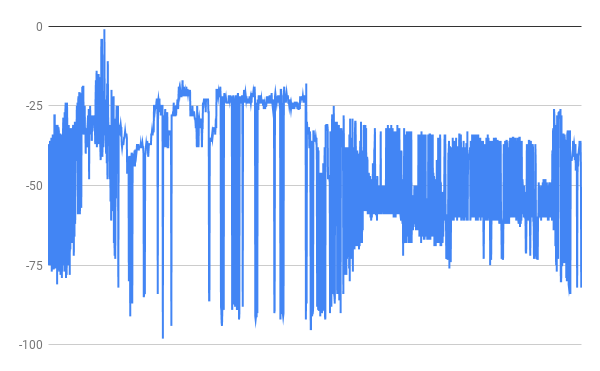
\includegraphics[scale=0.3]{WLAN/chart.png} 
\end{center}

Siempre está en el canal 11 excepto en el paquete 322, que está en el 6, como podemos comprobar:

\begin{center}
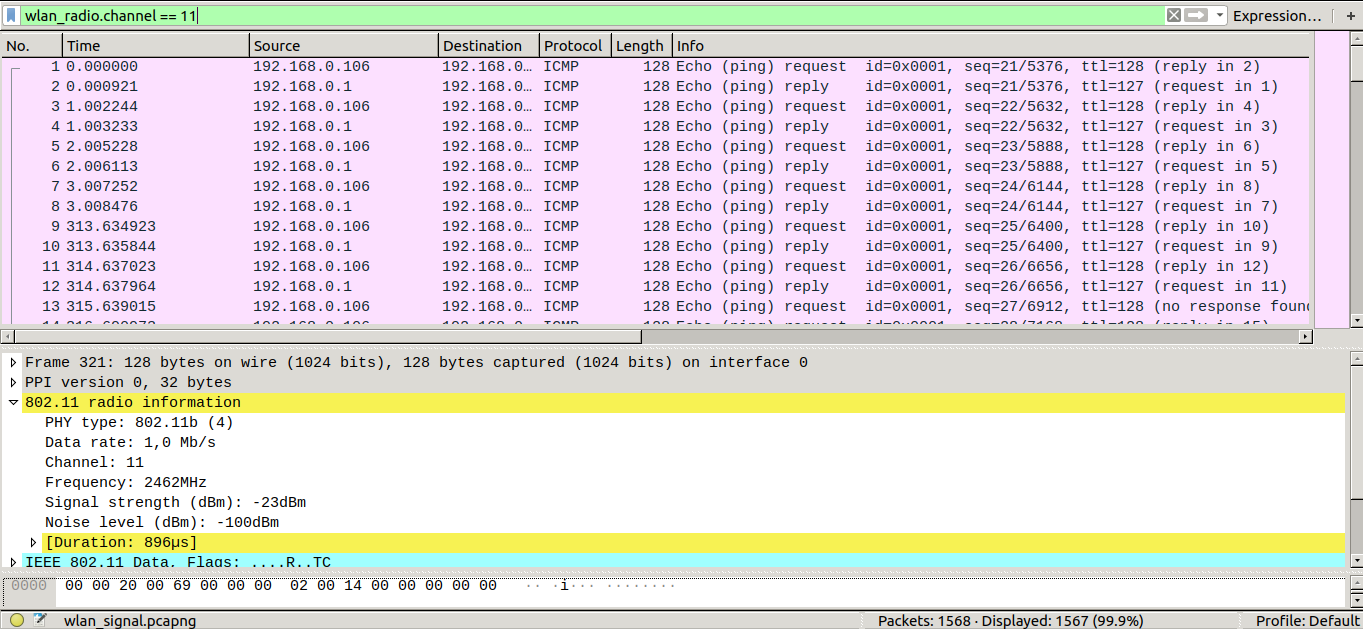
\includegraphics[scale=0.3]{WLAN/channel11.png} 
\end{center}

\begin{center}
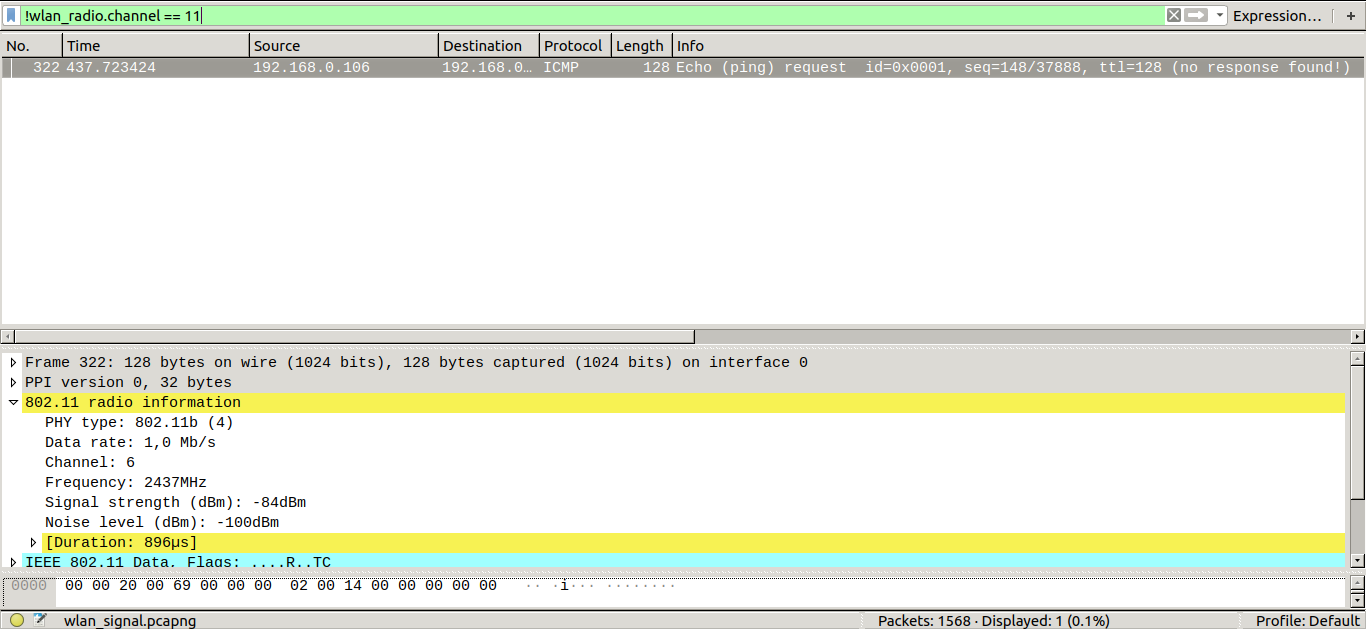
\includegraphics[scale=0.3]{WLAN/channel6.png} 
\end{center}

\section{Quiz 3}

En este ejercicio el problema es que ciertos paquetes tienen errores en con el checksum o el payload.

\begin{center}
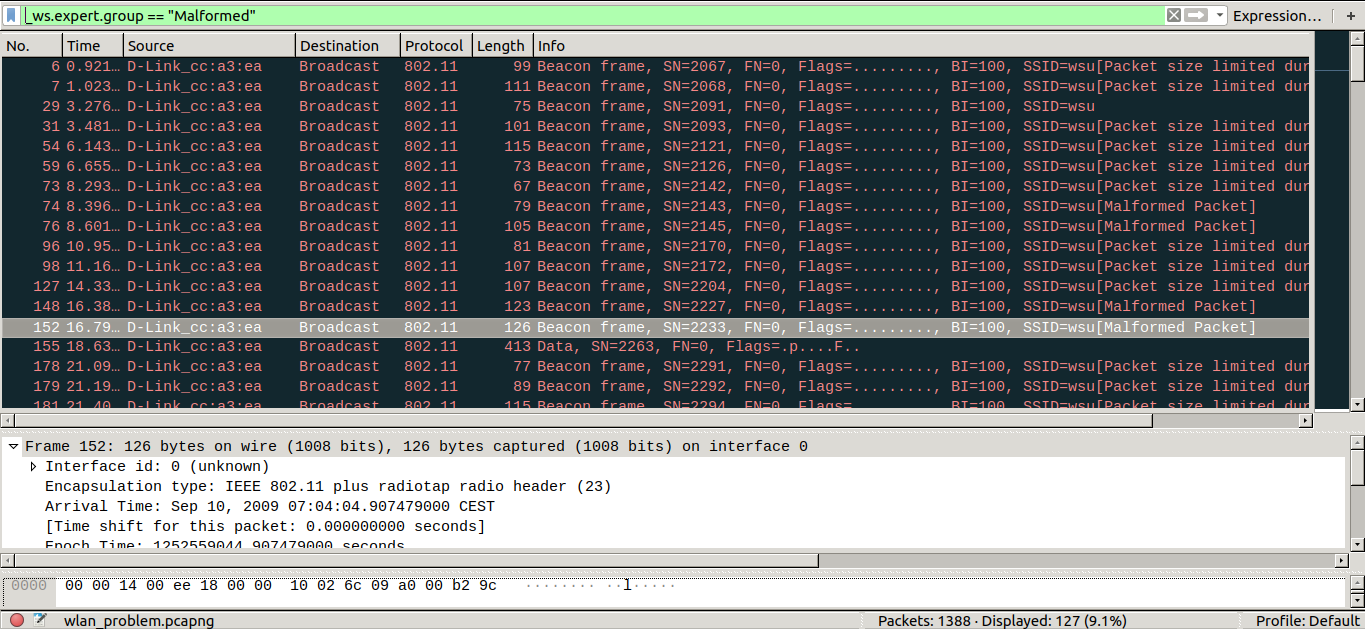
\includegraphics[scale=0.3]{WLAN/malformed.png} 
\end{center}

El tráfico es todo 802.11:

\begin{center}
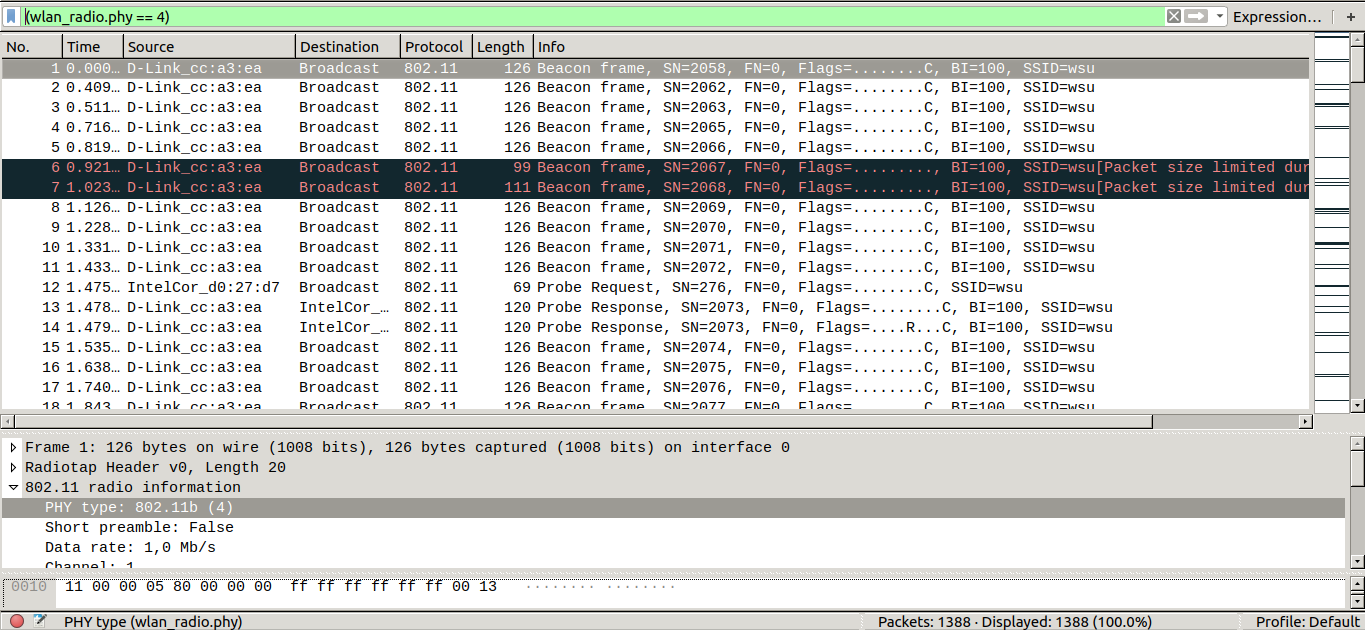
\includegraphics[scale=0.3]{WLAN/802_11}
\end{center}
\begin{center}
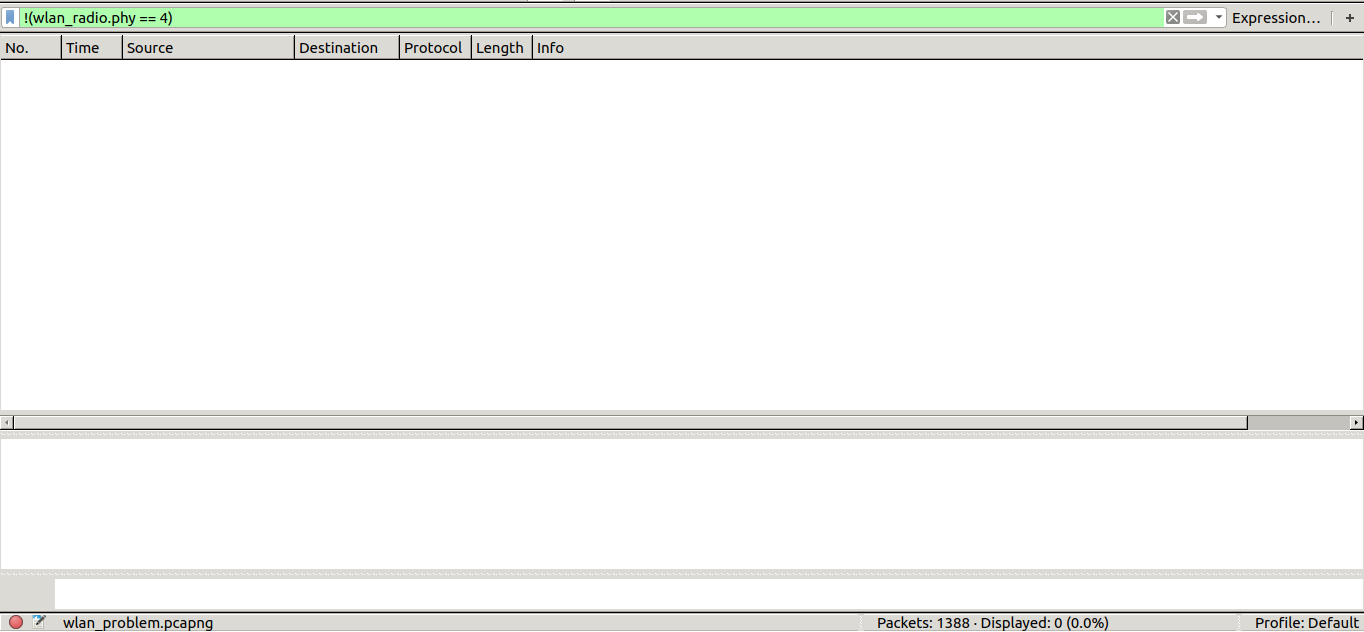
\includegraphics[scale=0.3]{WLAN/not802_11}
\end{center}

Todo el tráfico coloreado de blanco es de tipo broadcast (802.11) y el negro de tipo error en el checksum.

\begin{center}
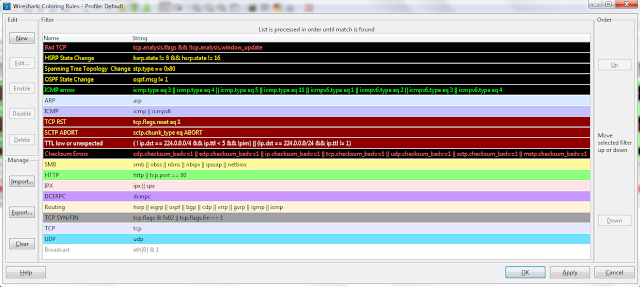
\includegraphics[scale=0.6]{WLAN/documentacion.png} 
\end{center}

\begin{thebibliography}{9}

\bibitem{Colores} \textit{Coloring rules}, \url{http://manualwireshark.blogspot.com/}.

\end{thebibliography}

\end{document}